%%%%%%%%%%%%%%%%%%%%%%%%%%%%%%%%%%%%%%%%%%%%%%%%%%%%%%%
% % Lines starting with % are comments, which are ignored.
% % This is a handy way of indicating the date and version of
% % your document, to wit:
% %
% % LaTeX sample file
% % Modified March, 2002
% %
%%%%%%%%%%%%%%%%%%%%%%%%%%%%%%%%%%%%%%%%%%%%%%%%%%%%%%%
\DocumentMetadata{
  % PDF standards: ONE key whose value is a comma-separated list --
  % UA-2 (accessibility) plus A-4f (archival; the archival companion of
  % UA-2). Do NOT use separate pdfstandard=... keys: with ordinary
  % key-value parsing only the last one takes effect.
  pdfstandard={UA-2,A-4f},
  lang=en-US,
  tagging=on,
  tagging-setup={
    math/setup=mathml-SE
  }
}

\documentclass{ltx-talk}
% lecture-macros.tex -- shared package setup for lecture-template.tex
% (ltx-talk slides / handouts).
%
% NOTE ON PATHS: every template in this repository is stored one level up
% from where it is compiled (see README.md). All relative \input paths
% below are resolved against the folder the document is compiled in,
% which sits one directory above this file.

% --- Tables, bookmarks, strikethrough ------------------------------------
% booktabs: professional table rules (\toprule, \midrule, \bottomrule)
% bookmark: PDF outline entries (PDF bookmarks)
% ulem[normalem]: \sout strikethrough that survives math mode
\usepackage{booktabs}
\usepackage{bookmark}
\usepackage[normalem]{ulem}
\usepackage{multicol}

% --- Math ------------------------------------------------------------
% amsmath: equation environments and numbering
% mathrsfs: \mathfrak  |  stmaryrd: extra symbols
\usepackage{amsmath}
\usepackage{mathrsfs}
\usepackage{stmaryrd}

% --- Layout -------------------------------------------------------------
% float: [H] float placement
% fontspec: Unicode/OpenType fonts (compile with XeLaTeX or LuaLaTeX)
\usepackage{float}
\usepackage{fontspec}

% --- Colors ---------------------------------------------------------------
% dvipsnames: extended named color palette (the Accessible* colors below
% are built on it);
% table: \rowcolors / \cellcolor for shading tables.
% NOTE: xcolor may only be loaded ONCE per document -- a second
% \usepackage{xcolor} with different options is a fatal "Option clash"
% error, so ALL of its options are listed here.
\usepackage[dvipsnames,table]{xcolor}

% --- Multimedia -----------------------------------------------------------
% animate: embeds audio/video (and legacy Flash) media in a frame.
\usepackage{animate}

% --- Bibliography ----------------------------------------------------------
% biblatex (biber backend): citations for lecture notes.
\usepackage[
  backend=biber,
  style=alphabetic,
  url=true,
  doi=true,
  isbn=true,
  backref=true
]{biblatex}

% --- Colored boxes ----------------------------------------------------------
% talkthemetcolorbox: the colored-box theme for ltx-talk slides
% (shadow/rounded/shaded blocks, showtitle, titlepage styles).
\usepackage[
  shadow,
  rounded,
  shaded,
  blocks,
  showtitle,
  titlepage
]{talkthemetcolorbox}

% --- "theindex" helper environment ------------------------------------------
% Provides a lightweight theindex environment (an itemize) and the
% \@idxitem/\subitem/\subsubitem/\indexspace macros that LaTeX's standard
% theindex machinery expects, so hand-written index pages indent correctly.
\makeatletter
\newenvironment{theindex}
  {\begin{itemize}}
  {\end{itemize}}
\providecommand\@idxitem{\par\hangindent 40\p@}
\providecommand\subitem{\@idxitem \hspace*{20\p@}}
\providecommand\subsubitem{\@idxitem \hspace*{30\p@}}
\providecommand\indexspace{\par \vskip 10\p@ \@plus5\p@ \@minus3\p@\relax}
\makeatother

% --- Index -----------------------------------------------------------------
% imakeidx: builds the printed index.
% The redefinition below appends "|hyperpage" to every index entry so that,
% in the PDF, each index entry is a link to its page.
\usepackage{imakeidx}
\makeatletter
\let\imki@orig@wrindexentrysplit\imki@wrindexentrysplit
\renewcommand\imki@wrindexentrysplit[3]{%
  \imki@orig@wrindexentrysplit{#1}{#2|hyperpage}{#3}%
}

\makeatletter
% --- Section titles: capture + one bookmark per logical section -------------
% \section is redefined so that:
%   1. the section title is captured into the plain-TeX register
%      \mytalksectitletoks (reprinted verbatim on the auto divider frame,
%      see the cmd/section/after hook below -- plain-TeX storage is
%      catcode-safe, unlike expanding the title in a hook), and
%   2. exactly ONE depth-1 PDF bookmark is created per \section call
%      (hyperref's own bookmark is suppressed via \Hy@writebookmark).
\DeclareCommandCopy{\OriginalSectionForBookmarks}{\section}
\newtoks\mytalksectitletoks

\RenewDocumentCommand{\section}{s o m}{%
  \begingroup
    \def\Hy@writebookmark##1##2##3##4##5{}%
    \global\mytalksectitletoks={#3}%
    \IfBooleanTF{#1}
      {\phantomsection\IfNoValueTF{#2}{\OriginalSectionForBookmarks*{#3}}{\OriginalSectionForBookmarks*[#2]{#3}}}%
      {\IfNoValueTF{#2}{\OriginalSectionForBookmarks{#3}}{\OriginalSectionForBookmarks[#2]{#3}}}%
  \endgroup
  \IfBooleanTF{#1}
    {\IfNoValueTF{#2}{\pdfbookmark[1]{#3}{section-star.\thepage.\number\inputlineno}}{\pdfbookmark[1]{#2}{section-star.\thepage.\number\inputlineno}}}%
    {\IfNoValueTF{#2}{\pdfbookmark[1]{Section \thesection: #3}{section.\thesection}}{\pdfbookmark[1]{Section \thesection: #2}{section.\thesection}}}%
}
\makeatother

% --- One PDF bookmark per logical frame (NOT per overlay) ---------------------
% ltx-talk writes one PDF page per overlay, so a naive frametitle hook would
% register a new bookmark for every overlay of the same frame. The
% \g_slideutils_frame_bookmark_int register remembers the last frame that
% got a bookmark, so subsequent overlays of the same frame are skipped.
% This is also what keeps BeamerPresenter's cumulative annotations working:
% one logical frame must stay one logical unit in the PDF outline.
\ExplSyntaxOn
\int_new:N \g_slideutils_frame_bookmark_int

\AddToHook{cmd/frametitle/after}{%
  \tl_if_empty:NF \g__talk_frame_title_tl
    {
      \ifnum\value{frame}=\g_slideutils_frame_bookmark_int\relax
      \else
        \int_gset:Nn \g_slideutils_frame_bookmark_int { \value{frame} }%
        \pdfbookmark[2]{\tl_use:N \g__talk_frame_title_tl}
          {frame.\int_use:N \g_slideutils_frame_bookmark_int}
      \fi
    }
}
\ExplSyntaxOff
\makeatother

% --- Printed index + theme for the colored boxes -------------------------------
% \makeindex[...]: two-column index titled "Index", listed in the TOC.
% The two EditInstance calls style the standard header/footer instances
% of talkthemetcolorbox (cyan background; footer order title/author/
% date/framenumber).
\makeindex[columns=2, title=Index, intoc]\EditInstance{header}{std}{
  background-color = cyan,
  color            = black,
  height           = 0.75cm
}
\EditInstance{footer}{std}{
  background-color = cyan,
  element-order = {title, author, date, framenumber},
}

% --- Auto section divider frame ---------------------------------------------------
% After each \section, insert a centered, large, structure-colored frame
% that prints the section title (from \mytalksectitletoks).
\AddToHook{cmd/section/after}{%
  \begin{frame}
    \centering
    \color{structure}
    \LARGE
    \the\mytalksectitletoks
  \end{frame}%
}

% --- Tagging sockets (tagged PDF structure) ---------------------------------------
% ltx-talk exposes tagging "sockets" where the PDF structure can attach
% section titles; register one and leave it unassigned (none) so the
% class's own tagging keeps control.
\ExplSyntaxOn
\AtBeginDocument{
  \NewTaggingSocketPlug { talk / sec / title } { none } { }
  \AssignTaggingSocketPlug { talk / sec / title } { none }
}
\ExplSyntaxOff

% --- Accessibility roles ----------------------------------------------------------------
% Map \frametitle to the H1 heading role in the tagged PDF, so screen
% readers treat slide titles as headings.
\tagpdfsetup{role / new-tag = frametitle / H1}

\makeatletter
% --- Page label = frame number -------------------------------------------------------
% Redefine what feeds the PDF page label to track the frame counter,
% not the physical page counter. Replace \theframenumber below with
% whatever internal macro/property ltx-talk actually uses to produce
% the "framenumber" footer element — confirm via ltx-talk-frame.dtx.
\renewcommand\thepage{\arabic{frame}}
\makeatother

\addbibresource{refs.bib}

% --- "Problem Time!" slides ------------------------------------------------------------------
% \ProblemSlide{problem}{solution} emits two frames: the problem, then
% its solution after a \pause, each numbered by the problem counter.
\newcounter{problemcounter}
\setcounter{problemcounter}{0}
\newcommand{\ProblemSlide}[2]{
  \stepcounter{problemcounter}
  \begin{frame}
    \frametitle{Problem Time!}
    Problem \theproblemcounter: #1
  \end{frame}

  \begin{frame}
    \frametitle{Problem Time!}
    Solution to Problem \theproblemcounter: \pause

    #2
  \end{frame}
}
% \highlight[<colour>]{<stuff>}
% from https://tex.stackexchange.com/questions/33401/a-version-of-colorbox-that-works-inside-math-environments
\newcommand{\highlight}[2][yellow]{\mathchoice%
  {\colorbox{#1}{$\displaystyle#2$}}%
  {\colorbox{#1}{$\textstyle#2$}}%
  {\colorbox{#1}{$\scriptstyle#2$}}%
  {\colorbox{#1}{$\scriptscriptstyle#2$}}}%

% --- Fonts ------------------------------------------------------------------------------
% Lato (text) + LeteSansMath (math): open, accessible typefaces.
\setmainfont{Lato}[
  Ligatures=TeX,
  Numbers={Lining,Monospaced}
]
\setsansfont{Lato}[
  Ligatures=TeX,
  Numbers={Lining,Monospaced}
]
\setmathfont{LeteSansMath.otf}\usepackage{emoji}

% --- Accessible colors ---------------------------------------------------------------------
% WCAG-contrast-safe variants of red/green for text on white:
% red!80!black and green!40!black both clear the 4.5:1 requirement.
% AltYellow: soft background for highlight boxes.
\colorlet{AccessibleRed}{red!80!black}
\colorlet{AccessibleGreen}{green!40!black}
\definecolor{AltYellow}{RGB}{255,245,170}

% --- Links ---------------------------------------------------------------------------------
% hyperref + link colors: every link uses AccessibleGreen (7.2:1 on
% white), so internal, citation, and URL links all pass WCAG 1.4.3.
\usepackage{hyperref}
\hypersetup{
  colorlinks=true,
  linkcolor=AccessibleGreen,
  urlcolor=AccessibleGreen,
  citecolor=AccessibleGreen,
}

% --- Shared course macros ---------------------------------------------------------------------
% Root macros.tex: math shorthands used across all course documents
% (\RR, \NN, \ZZ, \QQ, \grad, \curl, \tr, \der, \pder, ...).
\newcommand{\RR}{\mathbb{R}}
\newcommand{\NN}{\mathbb{N}}
\newcommand{\ZZ}{\mathbb{Z}}
\newcommand{\QQ}{\mathbb{Q}}
\newcommand{\vv}{\vec{v}}
\newcommand{\ww}{\vec{w}}
\newcommand{\xx}{\vec{x}}
\newcommand{\yy}{\vec{y}}
\newcommand{\zz}{\vec{z}}
\newcommand{\uu}{\vec{u}}
\newcommand{\basis}[1]{\vec{e_{#1}}}
\newcommand{\id}{\mathrm{id}}
\newcommand{\CC}{\mathbb{C}}
\renewcommand{\div}{\operatorname{div}}
\newcommand{\grad}{\operatorname{grad}}
\newcommand{\curl}{\operatorname{curl}}
\newcommand{\tr}{\operatorname{tr}}
\newcommand{\der}[2]{\dfrac{d #1}{d #2}}
\newcommand{\pder}[3][]{\dfrac{\partial^{#1} #2}{\partial #3}}


% % Title and author(s)
%%%%%%%%%%%%%%%%%%%%%%%%%%%%%%%%%%%%%%%%%%%%%%%%%%%%%%%
\title{Lecture 15 - Optimization I: The First Derivative Test}
\author{Garrett Credi}
\date{10/29/2026}
%%%%%%%%%%%%%%%%%%%%%%%%%%%%%%%%%%%%%%%%%%%%%%%%%%%%%%%
% %
% % The next command allows your in import encapsulated
% % postscript files, .epsf or .eps files, which
% % contain vector graphic image data.
% %
%%%%%%%%%%%%%%%%%%%%%%%%%%%%%%%%%%%%%%%%%%%%%%%%%%%%%%%
% %   The first thanks indicates your affiliation
% %
% %  Just the name here.
% %
% % Your mailing address goes at the end.
% %
% % \thanks is also how you indicate grant support
% %
%%%%%%%%%%%%%%%%%%%%%%%%%%%%%%%%%%%%%%%%%%%%%%%%%%%%%%%

%%%%%%%%%%%%%%%%%%%%%%%%%%%%%%%%%%%%%%%%%%%%%%%%%%%%%%%
% $ The next command ensures the margins are 1 inch on
% % all sides.
% %
%%%%%%%%%%%%%%%%%%%%%%%%%%%%%%%%%%%%%%%%%%%%%%%%%%%%%%%
\begin{document}
\begin{frame}
  \maketitle
\end{frame}

\begin{frame}
  \frametitle{Updates}

  Grading taking longer than expected, my apologies!

  Review Session: 4:30-6:30 in Vincent Hall 16 (the auditorium in the basement of Vincent). This place is HUGE so feel free to invite your friends in other sections of 1271 to come.

  Today's lecture content will \textit{\textbf{NOT}} be tested on Exam 2, it is Exam 3 content.
\end{frame}

\begin{frame}
  \frametitle{Quiz Time!}

  Let's get into neat rows, spread out, and slay this quiz!
\end{frame}

\section{Optimization}
\begin{frame}
  \frametitle{Derivative Review}

  Today's content arguably the \textit{most important} application of the derivative, \pause as such let's review some key facts about the derivative. \pause

  \begin{enumerate}
    \item The \textit{first} derivative of $f(x)$ at $x = x_0$ is the slope of the best linear approximation (linearization) at $x = x_0$: \pause
      \begin{equation}
        \mathscr{L}_{x = x_0}(x) = f(x_0) + f'(x_0)(x - x_0)
      \end{equation} \pause
    \item As such, the \textit{first} derivative is related to increasingness/decreasingness by: \pause $f(x)$ increasing/decreasing at $x = x_0$ $\iff$ $f'(x_0)$ is positive/negative. \pause
    \item Curvature of $f(x)$ at $x = x_0$ is controlled by \pause the sign of the \textit{second} derivative $f''(x_0)$: \pause concave up/down $\iff$ $f''(x_0)$ positive/negative \pause
    \item Comes from \textit{best quadratic approximation}:
      \begin{equation}
        \mathscr{Q}_{x = x_0}(x) = f(x_0) + f'(x_0)(x - x_0) + \dfrac{f''(x_0)}{2}(x - x_0)^2
      \end{equation}
  \end{enumerate}
\end{frame}

\begin{frame}
  \frametitle{Towards Optimization}

  After modelling some real world relationship as a function $output = f(input)$, one often wants to find the perfect input quantity that
  maximizes/minimizes the output quantity. \pause

  E.g.:
  \begin{itemize}
    \item If the relationship is: input=characteristic of material, output=cost of producing material with that characteristic then companies often want to \textit{minimize} \pause
    \item If the relationship is: input=cost of R\&D and output=net profit from R\&D companies often want to \textit{maximize} \pause
    \item If input=pH of substrate and output=reaction rate then both maxima and minima tell you important information about the chemical process. \pause
  \end{itemize}
\end{frame}

\begin{frame}
  \frametitle{Optimization Defns. I}
  To mathematically model this type of behavior we need to lay down a few defns. \pause

  \begin{block}{Global Minima/Maxima/Extrema}\index{extrema!global}\index{maxima!global}\index{minima!global}
    Given a function $f(x)$, we say that an \textit{output value} $f(c)$
    is a \textit{global} minimum/maximum resp. if, \pause for any other input $x_0$ in the domain of $f(x)$ \pause, $f(c)$ is $\leq/\geq$ resp. than $f(x_0)$. \pause

    If $f(c)$ is \textit{either} a global minimum/global maximum we call it a global \textit{extremum}.
  \end{block} \pause

  This is fantastic for real world applications, but derivatives struggle
  to classify these because the derivative is something defined
  locally only to a point. \pause This (hopefully) motivates us to adapt the above definition to something more \textit{local}.
\end{frame}

\begin{frame}
  \frametitle{Optimization Defns. II}

  \begin{block}
    {Local Minima/Maxima/Extrema}\index{extrema!local}\index{maxima!local}\index{minima!local}
    Given a function $f(x)$, we say that an \textit{input/output pair} $(c, f(c))$ is a \textit{global} minimum/maximum resp. if, \pause
    there is some small neighborhood $(c - \epsilon, c + \epsilon)$ around $c$, for which any $c - \epsilon < x_0 < c + \epsilon$, \pause $f(c)$ is $\leq/\geq$ resp. than $f(x_0)$. \pause

    If $(c, f(c))$ is \textit{either} a local minimum/local maximum we call it a local \textit{extremum}.
  \end{block} \pause

  Given how similar the defns. are, these two concepts are very tightly related: \pause
  \begin{alertblock}{Global Extrema are Local Extrema}\index{maxima!global!are local maxima}\index{minima!global!are local minima}\index{extrema!global!are local extrema}
    If $f(c)$ is a global minimum/maximum/extremum then $(c, f(c))$
    is a local minimum/maximum/extremum.
  \end{alertblock}
\end{frame}

\begin{frame}
  \frametitle{Optimization Defns. Example}
  Let's differentiate (pun maybe intended) the two defns. by examining
  the wavy function $f(x) = \dfrac{\sin(x)}{x}$: \pause

  \begin{figure}
    \centering
    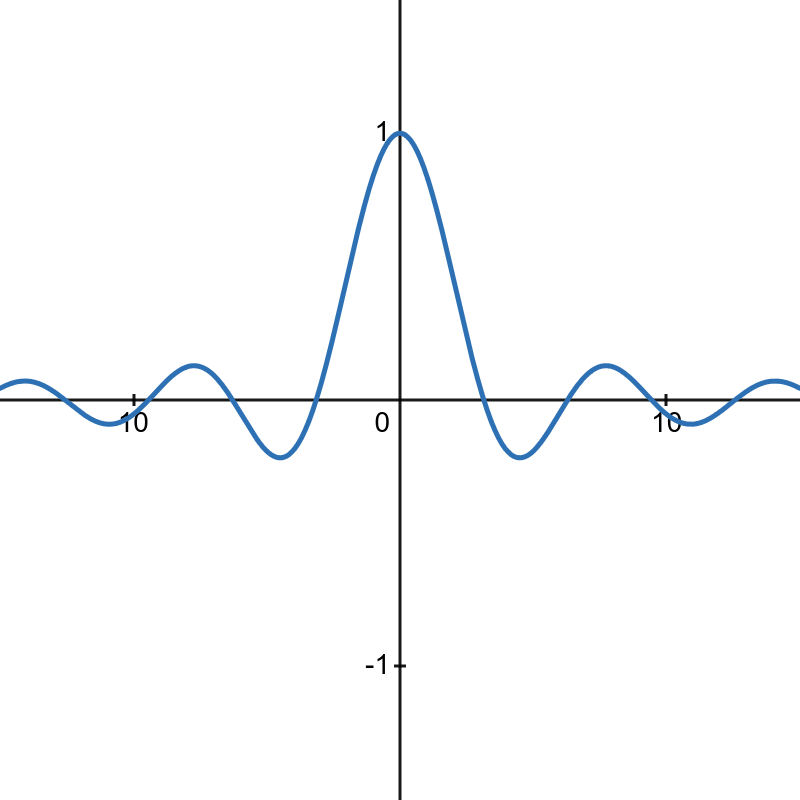
\includegraphics[height=0.6\textheight]{sinxoverx.png}
    \caption{Graph of $\dfrac{\sin(x)}{x}$}
  \end{figure}
\end{frame}

\begin{frame}
  \frametitle{Optimization I}

  If we want to use calculus tools to help us find local/global extrema, \pause
  we should first figure out what tools of ours actually contain enough information to detect local/global extrema in the first place. \pause

  In English: \pause which of our approximations actually themselves have local/global extrema \pause that are \textit{related} to those of the original function? \pause

  Attempt 1: Linearization. \pause Do linearizations have local/global extrema, can they recognize those in the original function? \pause

  \begin{figure}
    \centering
    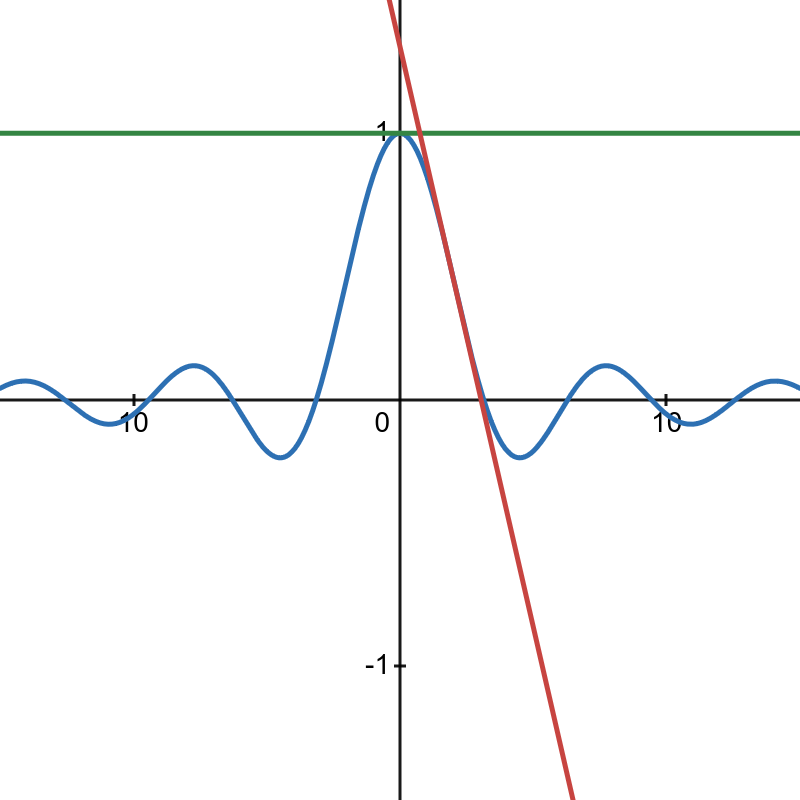
\includegraphics[height=0.4\textheight]{sinxoverx-linearization.png}
    \caption{Graph of $\dfrac{\sin(x)}{x}$ with two linearizations graphed.}
  \end{figure}
\end{frame}

\begin{frame}
  \frametitle{Optimization II}
  Lines suck! \pause Everything or nothing is an extrema, which makes us sad. \pause Let's bump it up to quadratic approximations. \pause

  \begin{figure}
    \centering
    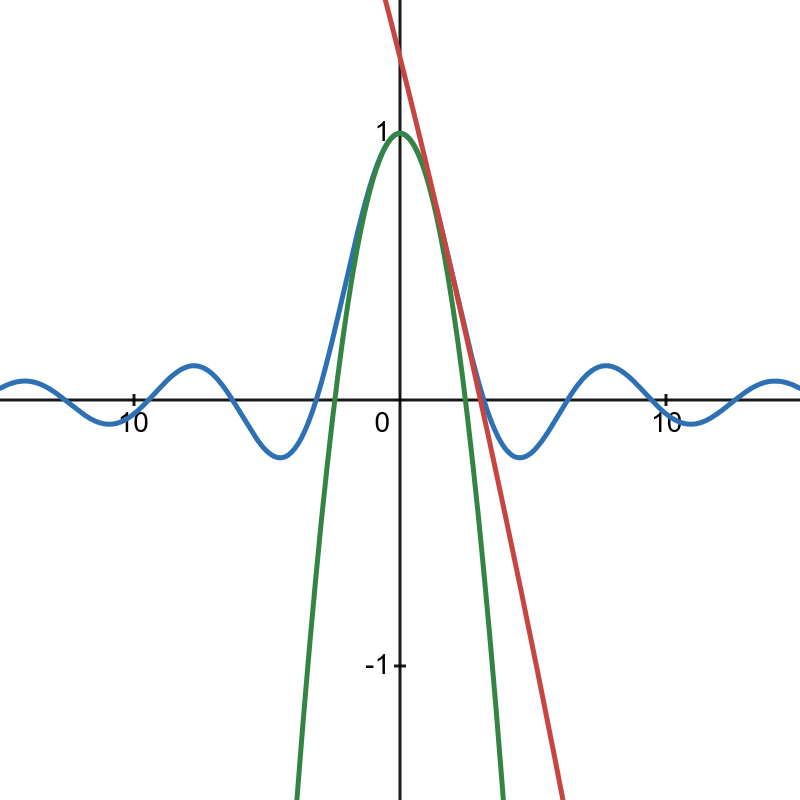
\includegraphics[height=0.6\textheight]{sinxoverx-quadratic.png}
    \caption{Graph of $\dfrac{\sin(x)}{x}$ with two quadratic approximations graphed.}
  \end{figure}
\end{frame}

\begin{frame}
  \frametitle{Optimization III}
  Quadratic approximations detect extrema! \pause
  The extrema for parabola occurs at their \pause vertex, \pause
  and the vertex of $f(x_0) + f'(x_0)(x - x_0) + \dfrac{f''(x_0)}{2}(x-x_0)^2$ is at $(x_0, f(x_0))$ if and only if \pause $f'(x_0) = 0$!
  
  If this seems weird, let's take what we've learned and reinterpret it in a much more direct manner: \pause
  \begin{enumerate}
    \item We needed to take a quadratic approximation at $x = x_0$, \pause this means that $f(x)$ has what property? \pause $f(x)$ is second differentiable at $x = x_0$. \pause
    \item The quantity $f'(x_0)$ was important; if $f(x)$ is second differentiable at $x = x_0$ what does that imply about $f'(x)$ at $x = x_0$? \pause $f(x)$ is continuously differentiable at $x = x_0$! \pause
    \item Can we rephrase the condition being a local minimum/maximum in this setting to relate it to conditions on the derivative? \pause Yes!
  \end{enumerate}
\end{frame}

\begin{frame}
  \frametitle{Optimization IV}
  Let's assume that $f(x)$ is a function that is both continuously differentiable at $x = x_0$ and that has a local extrema at $(x_0, f(x_0))$.

  If we have a local \textit{minimum} at $x = x_0$ then:
  \begin{itemize}
    \item If $x_0 - \epsilon < x \leq x_0$ (to the left of $x_0$) then what can we say about $f(x_0)$, $f(x)$ and $f'(x_0)$? \pause Minimality implies $f(x_0) < f(x)$ and so \pause
      by mean value theorem, $f'(x) \leq 0$ for $x_0 - \epsilon < x < x_0$. \pause 
    \item If $x_0 \leq x < x_0 + \epsilon$ (to the right of $x_0$) then what can we say? \pause Minimality implies $f(x_0) < f(x)$ so by MVT $f'(x) \geq 0$. \pause
    \item If $f'(x) \leq 0$ for $x < x_0$, $f'(x) \geq 0$ for $x > x_0$ \textit{AND} $f'(x)$ is continuous at $x = x_0$, then that forces $f'(x_0) \pause = 0$!
  \end{itemize} \pause

  Moral of the story: At a minimum, we start decreasing (negative derivative) then increase (positive derivative) \pause which forces the derivative at the switching point $f'(x_0)$ to be zero.

  Exercise: think about what happens when instead $(x_0, f(x_0))$ is a local \textit{maximum}.
\end{frame}

\begin{frame}
  \frametitle{Optimization V}

  We can compile this into the following important result:

  \begin{alertblock}{First Derivative Test}\index{optimization!first derivative test}\index{extrema!local!first derivative test}
    If $(x_0, f(x_0))$ is a local extremum (or global extremum) \pause
    and $f(x)$ is continuously differentiable at $x = x_0$, \pause
    then we \textit{must} have $f'(x_0) = 0$.
  \end{alertblock} \pause

  Unfortunately, this does not \textit{perfectly} classify local extrema, even for the nicest (infinitely differentiable) functions: consider $f(x) = x^3$:

  \vfill
\end{frame}

\begin{frame}
  \frametitle{Optimization VI}
  This condition is so important we give it its own name:

  \begin{block}{Critical Point}\index{critical point}\index{optimization!critical point}
    For a function $f(x)$ we say that $x_0$
    is a \textit{critical point} of $f(x)$ if $f'(x_0)$ is $0$ \pause or for
    technical reasons if $f'(x_0)$ is \textit{undefined}.
  \end{block} \pause

  The undefined condition is to handle functions like $f(x) = \sqrt[3]{x^2}$:
  \vfill
\end{frame}

\begin{frame}
  \frametitle{Optimization VII}
  Why do we care then?\pause

  Recall that solving equations like $f'(x) = 0$ often has us end up with
  a \textit{finite} set of points \pause and searching over a \textit{finite} set of points is MUUUCH easier than, for instance, searching over all of $\RR$ (super duper infinite).

  This gives us the following procedure: \pause in order to find the extrema of a function $f(x)$ we can avoid the futile task of comparing all the infinite values $f(c)$ for $c \in \RR$ by instead:
  \begin{itemize}\index{optimization!first derivative test!application procedure}
    \item Showing/recognizing that $f(x)$ is continuously differentiable \pause
    \item Solving for all the critical points of $f(x)$ \pause
    \item Computing $f(c)$ for every critical point $c$ \pause
    \item Comparing those above values to find the largest (maximum) and smallest (minimum). 
  \end{itemize}
\end{frame}

\begin{frame}
  \frametitle{Optimization Example I}
  Let's optimize the function $f(x) = \dfrac{x^5}{5} - \dfrac{x^4}{4} - \dfrac{2x^3}{3} + 2$! \pause

  We first find the critical points: \pause
  \begin{align}
    f'(x) &= x^4 - x^3 + 2x^2 \\ \pause
          &= x^2(x^2 - x + 2) \\ \pause
          &= x^2(x - 2)(x + 1)
  \end{align} \pause

  So we have critical points at $x = 0, 2, -1$. \pause

  But are they extrema? \pause I.e. in addition to having $f'(c) = 0$ does \pause $f'(c)$ actually switch signs at $x = c$?
\end{frame}

\begin{frame}
  \frametitle{Optimization Example II}
  This is where the notion of a sign graph comes in:

  \begin{block}{Sign Graph}\index{sign graph}\index{optimization!sign graph}
    Given a function $f(x)$, the sign graph of $f(x)$ is a useful way to depict only the positivity or negativity of a function. \pause

    We start with drawing out the domain of $f(x)$ as a number line, \pause
    mark each $x$ value where $f(x) = 0$ or is undefined, \pause
    and then (assuming $f(x)$ is continuous) \pause can characterize
    the sign over each split interval just by evaluating at a single point.
  \end{block} \pause

  \vfill
\end{frame}

\begin{frame}
  \frametitle{Optimization Example III}
  Thus we have that $f'(x)$ only switches signs across $x = 2$ and $x = -1$. \pause

  This means that:
  \begin{enumerate}
    \item $x = 0$ is \pause just a critical point, and not an extrema. \pause
    \item $x = 2$ is where the sign switches from \pause negative to \pause positive, so $x = 2$ is a \pause local minimum. \pause
    \item $x = -1$ is where the sign switches from \pause positive to \pause negative so $x = -1$ is a \pause local maximum.
  \end{enumerate} \pause

  Thus we've determined that, for $f(x) = \dfrac{x^5}{5} - \dfrac{x^4}{4} + \dfrac{2x^3}{3} + 2$, there is a local minimum at $x = 2$ and a local maximum at $x = -1$. \pause Check the graph, and we see that's correct!
\end{frame}

\begin{frame}
  \frametitle{Optimization Example IV}

  Let's instead consider $f(x) = x + \sqrt[3]{x^2}$. \pause

  We start by finding critical points:
  \begin{align}
    f'(x) &= 1 + \dfrac{2}{3\sqrt[3]{x}} \\ \pause
          &= \dfrac{2 + 3\sqrt[3]{x}}{3\sqrt[3]{x}}
  \end{align} \pause

  Which is zero when: \pause
  \begin{gather}
    2 + \sqrt[3]{x} = 0 \\ \pause
    \sqrt[3]{x} = -2 \\ \pause
    x = (-2)^3 = -8
  \end{gather} \pause

  and is undefined when: \pause
  \begin{gather}
    3\sqrt[3]{x} = 0 \\ \pause
    \sqrt[3]{x} = 0 \\ \pause
    x = 0^3 = 0
  \end{gather}
\end{frame}

\begin{frame}
  \frametitle{Optimization Example V}

  \vspace{\stretch{0.1}}
  We then construct the sign graph of $f'(x) = \dfrac{2 + 3\sqrt[3]{x}}{3\sqrt[3]{x}}$. \pause

  \vspace{\stretch{1}}

  Which gives us that at $x = -8$ the sign changes from \pause positive to \pause negative,

  and at $x = 0$ the sign changes from \pause negative to \pause positive. \pause

  Therefore $x = -8$ is a local \pause maximum, \pause
  and $x = 0$ is a local \pause minimum.
  \vspace{\stretch{0.1}}
\end{frame}

\begin{frame}
  \frametitle{Worksheet Time}

  Let's get into groups and work on the worksheet!
\end{frame}

\begin{frame}
  \frametitle{End of Class}

  That's all folks!
\end{frame}
\end{document}
